%% $RCSfile: using.tex,v $
%% $Revision: 1.1 $
%% $Date: 2010/04/23 01:57:05 $
%% $Author: kevin $
%%

\chapter{Work Done}\label{C:WorkDone}
This chapter presents a comprehensive description of the current status of the project. To complete objective one, we
designed a matrix-based representation for the service location-allocation problem. A Multi-objective PSO-based approach
is then proposed to solve the problem. The experimental results reveal the effectiveness and efficiency of our approach
in comparison with our previous NSGA-II-based approach.

\section{Problem Description , Assumptions and Modeling}
\label{sec:problem}
In this section, we first describe the service location-allocation problem, then we will present models for the services location-allocation problem.

\subsection{Problem Description}
Web service location-allocation problem is to determine reasonable locations for Web services so that the deployment cost of WSP can be minimized while service performance can be optimized.
In this paper, to optimize service performance we consider to minimize network latency.

The task of service location-allocation has two objectives:
\begin{itemize}
	\itemsep0em
	\item To minimize the total cost of the services.
	\item To minimize the total network latency of the services.
\end{itemize}


\subsection{Assumptions}
To model the service location-allocation problem, we consider the following assumptions.
%\begin{enumerate}
	%\item The new WSP decides where to locate his facilities regardless of there is existed functional similar services from other WSPs.
	%\item The decision of service location-allocation is made only considering two factors: total network latency and total cost.
	%\item A static allocation policy is used by WSPs. In practice, Web services typically offer clients persistent and interactive services, which often span over multiple sessions. Therefore, a dynamic reallocation scheme is not practical as it may disrupt the continuity of the services.
%\end{enumerate}
\subsubsection{Stakeholder Web Service Providers, User Centers and Candidate Locations}
Assume the historical information of Web service usage has been collected. WSPs wish to allocate services to servers in candidate locations in order to maximum their profit.

The WSP must decide on services locations from a finite set of possible locations. 
In order to make a decision, the WSP must first analyze the data collected from current use of services. 
The collected data should include the records of Web requests from each IP address.
Therefore, based on these data, the WSP could summarize customer demands concentrated on \textit{n} discrete nodes \cite{Aboolian}, namely user centers. 
We assume that the WSP has already done this step and a list of user centers and candidate 
locations are given. A candidate location is the geometric location that is suitable to 
deploy services. Candidate locations are selected based on other criterions such as 
facilities or deployment cost. User centers and candidate locations can be overlapping. In fact, 
Web serivce users receive best QoS services if the Web serivces are deployed locally.
Therefore, the WSPs would like to choose user centers as candidate locations.
In addition to deciding which locations to deploy, information about network latency between user centers and candidate locations are needed. 


The list below shows some critical information that should be providered by the WSPs.

\begin{enumerate}
	\itemsep0em
	\item A list of user centers
	\item A list of candidate locations
	\item Service invocation frequencies from user centers to services
	\item Average network latency from user centers to candidate locations
	\item Web service deployment cost for each candidate location
\end{enumerate}

Worth noting that service invocation frequencies are changing over time. For example, a 
service was popular in some regions may be unfrequented after a few months. That's the 
main reason for WSPs re-allocate their services. Network latency highly depends on the 
network traffic and may be very different during periods of a day. However, as long as 
there is no significant changes in the network topology, the average network latency
remain stable. Therefore, the average network latency for a period of time should be 
representative.

%These are the main input data that the decision making is dependent on. The details of 
%these input data and modeling are introduced in Section \ref{sec:model}. 
%Section \ref{sec:experiment} discussed the data that we used in the experiment.

\subsubsection{Static deployment vs. Dynamic deployment}
As virtual machine technology and infrastracture-as-a-service (IaaS) are becoming
more and more popular. Dynamic Web service deployment become possible \cite{kemps2012dynamic}. On the other hand, static deployment is still the mainstream because of a majority
of Web serivce are deployed on local infrastracture \cite{He}. In this paper, we made an
assumption that WSPs periodicaly change the Web service deployment since the user centers
are changing over time.


\subsection{Model Formulation}
To model service location-allocation problem, we need to make use of a set of matrices, to present input information and output solutions. 

For service location-allocation problem, we need information of service usage, network latency, and service deployment cost to decide service location-allocation so that the overall network latency can be minimized with minimal deployment cost and within constraints.
Assume a set of $S = \{ s_{1}, s_{2}, ...s_{s}, s_{x}\}$ services are
requested from a set of locations $I = \{ i_{1}, i_{2}, ...i_{i}, i_{y} \}$. 
The service providers allocate services to a set of candidate facility locations $J = \{ j_{1}, j_{2}, ...j_{j}, j_{z} \}$.


In this paper, we will use the following matrices.
\begin{center}
{
%\centering
	\begin{tabular}{l*{2}{l}r}
		\hline
		\textbf{Matrices} \cr
		$L$ & server network latency matrix $L = \{l_{ij}\}$ \cr
		$A$ & service location-allocation matrix $A = \{a_{sj}\}$ \cr
		%$A'$ & service location matrix $A' = \{a'_{sj}\}$ \cr
		$F$ & service invocation frequency matrix $F = \{f_{is}\}$ \cr
		$C$ & cost matrix $C = \{c_{sj}\}$ \cr
		$R$ & user response time matrix $R = \{r_{is}\}$ \cr
		\hline
	\end{tabular}
%\\
}
\end{center}
A \emph{service invocation frequency matrix}, $F= [f_{is}]$, is used to record services invocation frequencies from user centers, 
where $f_{is}$ is an integer that indicates the number of invocations in a period of time from a user center to a service. 
For example, $f_{13}$ = 85 denotes service $s_{1}$ is called 85 times in a predefined period of time.

\parbox{.45\linewidth}{
{\centering
$
F = \bbordermatrix{~ & s_{1} & s_{2} & s_{3}  \cr
					i_{1}	&120 &35 &56	\cr
					i_{2}	&14  &67 &24 \cr
					i_{3}	&85 &25 &74 \cr}
$
\\}
}
\parbox{.45\linewidth}{
{\centering
$
L = \bbordermatrix{~ & j_{1} & j_{2} & j_{3} \cr
					i_{1}	&0 &5.776 &6.984	\cr
					i_{2}	&5.776  &0 &2.035 \cr
					i_{3}	&0.984 &1.135	&2.3 \cr}
$
\\}
}

A \emph{network latency matrix} $L = [l_{ij}]$, is used to record network latencies from user centers to 
candidate locations. For example, the network latency between user center $i_{2}$ with candidate location $j_{1}$ 
is 5.776s. These data could be collected by monitoring network latencies \cite{6076756} \cite{5552800}.

The cost matrix, $C = [c_{sj}]$, is used to record the cost of deployment of services to candidate locations, 
where $c_{sj}$ is an integer that indicates the cost of deploying a service to a location. 
For example, $c_{12} = $ 80 denotes the cost of deploying service $s_{1}$ to location $j_{2}$ is 80 cost units.

\parbox{.45\linewidth}{
{\centering
$
C = \bbordermatrix{~ & j_{1} & j_{2} & j_{3}\cr
					s_{1}	&130 &80 &60\cr
					s_{2}	&96  &52 &86\cr
					s_{3}	&37 &25 &54\cr}
$
\\}
}
\parbox{.45\linewidth}{
{\centering
$
A = \bbordermatrix{~ & j_{1} & j_{2} & j_{3}\cr
					s_{1}	&0 &1 &0	\cr
					s_{2}	&0  &0 &1	\cr
					s_{3}	&1 &1 &0	\cr}
$
\\}
}

%\emph{service location-allocation matrix} $A = [a_{sj}]$ represents the actual service location allocation, where $a_{sj}$ is
%a binary value 1 or 0 to indicate whether a service is allocate to a location or not. 
%
%A' = \bbordermatrix{~ & j_{1} & j_{2} & j_{3}\cr
				%s_{1}	&0.12 &0.87 &0.42	\cr
				%s_{2}	&0.07  &0.32 &0.95	\cr
				%s_{3}	&0.76 &0.64 &0.27	\cr}

%\begin{equation}
	%\label{eq:1}
	%a'_{sj} = 
	%\begin{cases}
		%1 & \quad \text{if } a_{sj} > threshold \\
		%0 & \quad \text{otherwise} \\
	%\end{cases}
%\end{equation}

%The transformation threshold will be discussed in section \ref{}.


Using service location allocation matrix $A = [a_{sj}]$ and network latency matrix $L = [l_{ij}]$, we can compute user
response time matrix $R = [r_{is}]$, 

{\centering
	\begin{equation}
		r_{is} = MIN\{l_{ij} \mid j \in \{1, 2, ..., z\} \text{ and } a_{sj} = 1\}
	\end{equation}
\\}
For example, we can use the two example matrices $L$ and $A$ presented above to construct the response time matrix $R$. 
For each service $s$, by checking matrix $A$, we can find out which location the service has been deployed.
Then we check matrix $L$, to find out its corresponding latency to each user center $i$. If there is
more than one location, then the smallest latency is selected. Therefore, we can construct the response time matrix $R$ as:

{\centering
$
R = \bbordermatrix{~ & s_{1} & s_{2} & s_{3}\cr
					i_{1}	&5.776 &6.984 &0	\cr
					i_{2}	&0  &2.035 &0	\cr
					i_{3}	&1.135 &2.3 &0.984	\cr}
$
\\}

%\subsubsection{Summary}

%\begin{flushleft}\textbf{Input}:\end{flushleft}
%\begin{itemize}
	%\item \emph{L}: network latency from user centers to candidate locations
	%\item \emph{F}: service invocation frequency from user centers to Web services
	%\item \emph{C}: deployment cost for services in different candidate locations
%\end{itemize}

%\begin{flushleft}\textbf{Temporary variable}:\end{flushleft}
%\begin{itemize}
	%\item \emph{A}: service location-allocation probability matrix
%\end{itemize}

	
%\begin{itemize}
	%\item \emph{R}: user response matrix is a temporary variable generated during the optimization process
%\end{itemize}

%\begin{flushleft}\textbf{Output}:\end{flushleft}
%\begin{itemize}
	%\item \emph{A'}: the solution matrix
%\end{itemize}


\section{Multi-objective Particle Swarm Optimization with Crowding Distance for Web Service Location Allocation}
To apply MOPSOCD to the service location-allocation problem, the first step is to define variables in MOPSOCD (i.e., to
identify particle and the fitness functions).

\subsection{Particle Representation and Transformation Function}
EC algorithms generally treat output or desired solution (e.g., service location-allocation matrix $A$) as the 
``individual'' so that the solution evolve along with the process. However, in Web service location-allocation, the 
output is binary. It is not compatible with PSO.
In PSO, particles are ``flies'' in its own direction and velocity searching for a good solution in a continuous space. 
Therefore, the representation of particle is continuous.

We introduced a \emph{service location-allocation probability matrix}, $A' = [a'_{sj}]$ represents the probability of a 
service $s_{i}$ allocate to a candidate location $j_{i}$. 
$a'_{sj}$ is a real value, $a'_{sj} \in (0, 1)$ indicate the probability of a service is \textbf{NOT} 
allocate to a candidate location.

We use the service location-allocation probability matrix $A'$ = $[a'_{sj}]$ as a particle. 
During the PSO process, the particle needs to be transfered to binary representation in order to compatible with 
the modeling. In order to transfer $A' \rightarrow A$, we introduced a transformation
function.

\begin{equation}
	\label{eq:1}
	a_{sj} = 
	\begin{cases}
		1 & \quad \text{if } a'_{sj} > threshold \\
		0 & \quad \text{otherwise} \\
	\end{cases}
\end{equation}

The parameter $threshold$ is an empirical parameter that introduced into the algorithm. 

\subsection{Constraint}
In our case, we set one basic constraint. The service number constraint requires that each service is deployed in at 
least one location.

{
	\centering
	\begin{equation}
		\sum\limits_{x \in S} a_{xj} \geq 1
	\end{equation}
\\}

\subsection{Fitness Function}
\label{sec:fitness_functions}
\begin{flushleft}In order to accomplish these two objectives, we design two fitness functions to evaluate 
how good each particle meets the objectives. We use \emph{CostFitness} to calculate the overall cost of deploying services under an allocation plan\end{flushleft}
%\subsubsection{Cost fitness function}

%\vspace*{-1em}
\begin{equation}
	CostFitness = \sum\limits_{s \in S} \sum\limits_{j \in J} c_{sj} \times a_{sj}
\end{equation}

\begin{flushleft}where $c_{sj}$ is the cost of deploying service $s$ at candidate location $j$, $a_{sj}$ represents whether service $s$ is allocate to candidate location $j$. The sum of the multiplication of 
$c_{sj}$ and $a_{sj}$ is the total deployment cost.\end{flushleft}


%\begin{flushleft}For example, we use the above mentioned matrices $C$ and $A$.\end{flushleft}

	%$
	%CostFitness &= c_{11} * a_{11} + c_{12} * a_{12} + c_{13} * a_{13} + ... + c_{33} * a_{33} \\
	%&= 130 * 0 + 80 * 1 + 60 * 0 + ... + 54 * 0 \\
	%&= 228
	%$


We use \emph{LatencyFitness} to calculate the overall network latency. Where $r_{is}$ 
denotes the optima response time from a user center $i$ 
to a service $s$ and $f_{is}$ is the invocation frequency of a user center $i$ to a service
$s$.
	\begin{equation}
		LatencyFitness = \sum\limits_{i \in I} \sum\limits_{s \in S} r_{is} \times f_{is}
	\end{equation}

\begin{flushleft}For example, we use the above mentioned matrices $F$ and $R$.\end{flushleft}
	$
	LatencyFitness &= f_{11} * r_{11} + f_{12} * r_{12} + f_{13} * r_{13} + ... + f_{33} * r_{33} \\
	&= 120 * 5.776 + 6.984 * 35 + 0 * 56 + ... + 0.984 * 74\\
	&= 1300.696
	$

\subsubsection{Normalise function}
To indicate the goodness of an allocation solution we normalise \emph{CostFitness} and \emph{LatencyFitness} according to the largest and minimum values of
\emph{CostFitness} and \emph{LatencyFitness}. Normalised fitness values can also be used to compare results from different approaches.
Since the maximum and minimum values for total cost and total latency are deterministic, we use exhaustive search to
find out the $Latency_{max}$. $Latency_{min}$ is zero for we assume each service could be deployed in each user center. 
$Cost_{min}$ is the cost of allocating each of services at a location that leads to the minimal cost and $Cost_{max}$ is the cost of allocating each service is allocated to all the 
locations.
	\begin{equation}
		\label{eq:cost_prime}
		CostFitness^\prime = \frac{CostFitness - Cost_{min}}{Cost_{max} - Cost_{min}}
	\end{equation}

	\begin{equation}
		\label{eq:latency_prime}
		LatencyFitness^\prime = \frac{LatencyFitness - Latency_{min}}{Latency_{max} - Latency_{min}}
	\end{equation}


\subsection{MOPSOCD based algorithm for service location-allocation}
In this section we present our MOPSOCD based algorithm for service location-allocation as Algorithm 1.
\begin{algorithm}[htb]
	\caption{MOPSOCD for service location-allocation}
	\textbf{Inputs:}
		Cost Matrix $C$,
		Server network latency matrix $L$, 
		Service invocation frequency matrix $F$

	\textbf{Outputs:}
		Pareto Front: the $Archive$ set

	\begin{algorithmic}[1]
	\label{alg:1}
		\State Initialize a population $P$ with random real values $\in$ (0, 1)
		\State Each individual $i$ in $P$ using the fitness function
		\State Initialize personal best of each individual $i$.
		\State Initialize $GBEST$
		\State Initialize $Archive$ with nondominated vectors found in $P$

		\Repeat
			\State Compute the crowding distance values of each nondominated solution in the $Archive$
			\State Sort the nondominated solutions in $Archive$ in descending crowding distance values
			\For ( each particle)
				\State Update the $GBEST$ by randomly select a particle from top 10\% of $P$
				\State Compute the new velocity 
				\State Update its position
				\State If it goes beyond the boundaries, then multiply its velocity by -1
				\State If($t < (MAXT * PMUT)$), apply Mutation
				\State Evaluate fitness
				\State Update its $PBESTS$
				\EndFor
		\State Insert new nondominated solution into $Archive$, remove dominated solutions from $Archive$
		\Until{ maximum iterations is researched}
		\State return $Archive$
	\end{algorithmic}
\end{algorithm}


%\begin{algorithm}[htb]
	%\caption{NSGA-II for service location-allocation}
	%\label{NSGA2}
	%\textbf{Inputs:}
		%Cost Matrix $C$,
		%Server network latency matrix $L$, 
		%Service invocation frequency matrix $F$

	%\textbf{Outputs:}
		%Pareto Front:a  set of service allocation matrix $A$

	%\begin{algorithmic}[1]
		%\label{alg:2}
		%\State Initialize a population of chromosome with random binary values
		%\State Evaluate population with fitness functions
		%\State Non-dominated sort and assign a ranking to each chromosome
		%\State Evaluate the Crowding distance of each chromosome
		%\State Initialize the Pareto Front Pool
		%\While{predefined generation}
		%\State Apply Tournament Selection
		%\State Apply Crossover 
		%\State Apply Mutation
		%\For( each chromosome)
		%\While{ violate service number constraint}
		%\State random choose a location $j$ and set $a_{sj}$ = 1
		%\EndWhile
		%\While { violate cost constraint}
		%\State random choose a location $j$ and set $a_{sj}$ = 0, as long as $\sum\limits_{s \in S} a_{sj} \geq 1$
		%\EndWhile
		%\If{ chromosome does not exist in the Pareto front Pool}
		%\State Evaluate with the fitness functions
		%\EndIf
		%\EndFor
		%\State Non-dominated sort and assign ranking
		%\State Evaluate the Crowding distance
		%\State Recombination and Selection
		%\State Update the Pareto Front Pool with the current Pareto Front
		%\EndWhile
		%\State Return the Pareto Front
	%\end{algorithmic}
%\end{algorithm}

\section{Experimental Studies}

\subsection{Dataset}

Latency matrix was derived from WS-DREAM \cite{6076756, 5552800}, which is a 
historical dataset on QoS of Web services from different locations. It contains the data of latencies from 339 different
user locations invoked 5824 Web services scattered over different locations. 

A cost matrix is generated from a normal distribution with mean as 100 and standard deviation as 20. A frequency matrix 
is generated from a uniform distribution over [1, 120].


\subsection{Environment}

The algorithm was coded in R \cite{Morandat:2012:EDR:2367163.2367172} using existed packages: NSGA2R, MOPSOCD. 
The program was run on a 3.40GHz desktop computer with 8 GB RAM. 

\subsection{Test case}
Four different service location-allocation problems were designed with different complexities.

\begin{table}[h]
{\centering
	\caption{Test Cases}
	\begin{tabular}{|c|c|c|c|}
		\hline
		\multicolumn{1}{|l|}{problem} & \multicolumn{1}{l|}{number of service} & \multicolumn{1}{l|}{number of candidate location} & \multicolumn{1}{l|}{number of user center} \\\hline
		1                             & 20                                  & 5                                    & 10                                      \\\hline
		2                             & 50                                  & 15                                    & 20                                      \\\hline
		3                             & 100                                 & 25                                   & 40                                     \\\hline
		4                             & 200                                 & 40                                   & 80                                    \\
		\hline
	\end{tabular}
\\}
\end{table}


\subsection{Parameter}
Parameter settings for MOPSOCD are as follow. The population size is 50 and the maximum number of generations is 50.
The mutation rate $P_m$ is 0.5. The inertia parameter $w$ is 0.4. $c1$ and $c2$ are set to 1. The archive size is 250.
The transformation threshold is set to 0.7.

Parameter setting for NSGA-II are, population size is 50 and the maximum number of generations is 50. The tournament 
size is 3. The cross probability $P_c$ is 0.8 and the mutation probability $P_m$ is 0.2.

\subsection{Evaluation metrics}

To compare the result of MOPSOCD and NSGA-II, we first derive the Pareto front by using the approach in \cite{6381531, Xue}, and
then compare the results using approach in \cite{1688438}. In Xue's approach, 
40 sets of solution achieved by each multi-objective algorithm are firstly combined into one set. Secondly, we apply 
nondominated sort on each solution set and generated final solution set. 
Thirdly, we use cost fitness value and latency fitness value as x, y coordinate, plot the final solutions on a graph.
Our goal is to minimize both cost and latency. Therefore, better solution should locate closer to the origin.


\subsection{Experimental Results}
This section presents an analysis for the proposed MOPSOCD-based approach in solving the service location-allocation
problem. Figure \ref{fig:results} shows the experimental result for the four test cases.

%\begin{figure}[h!]
	%\centering
	%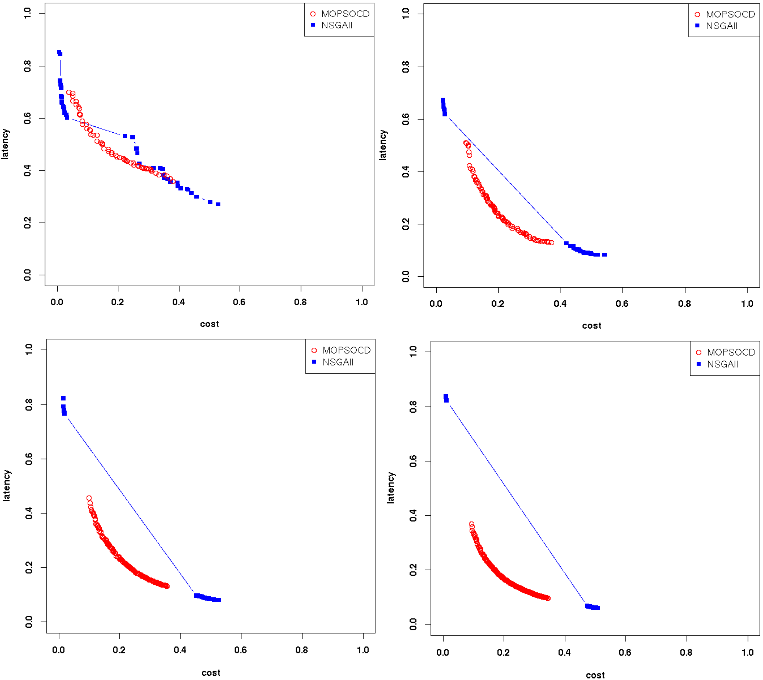
\includegraphics[width=0.9\textwidth]{pics/summary.png}
	%\caption{Experiments results}
	%\label{fig:results}
%\end{figure}

\begin{figure}[h!]
   \centering
   \begin{subfigure}{0.4\textwidth}
       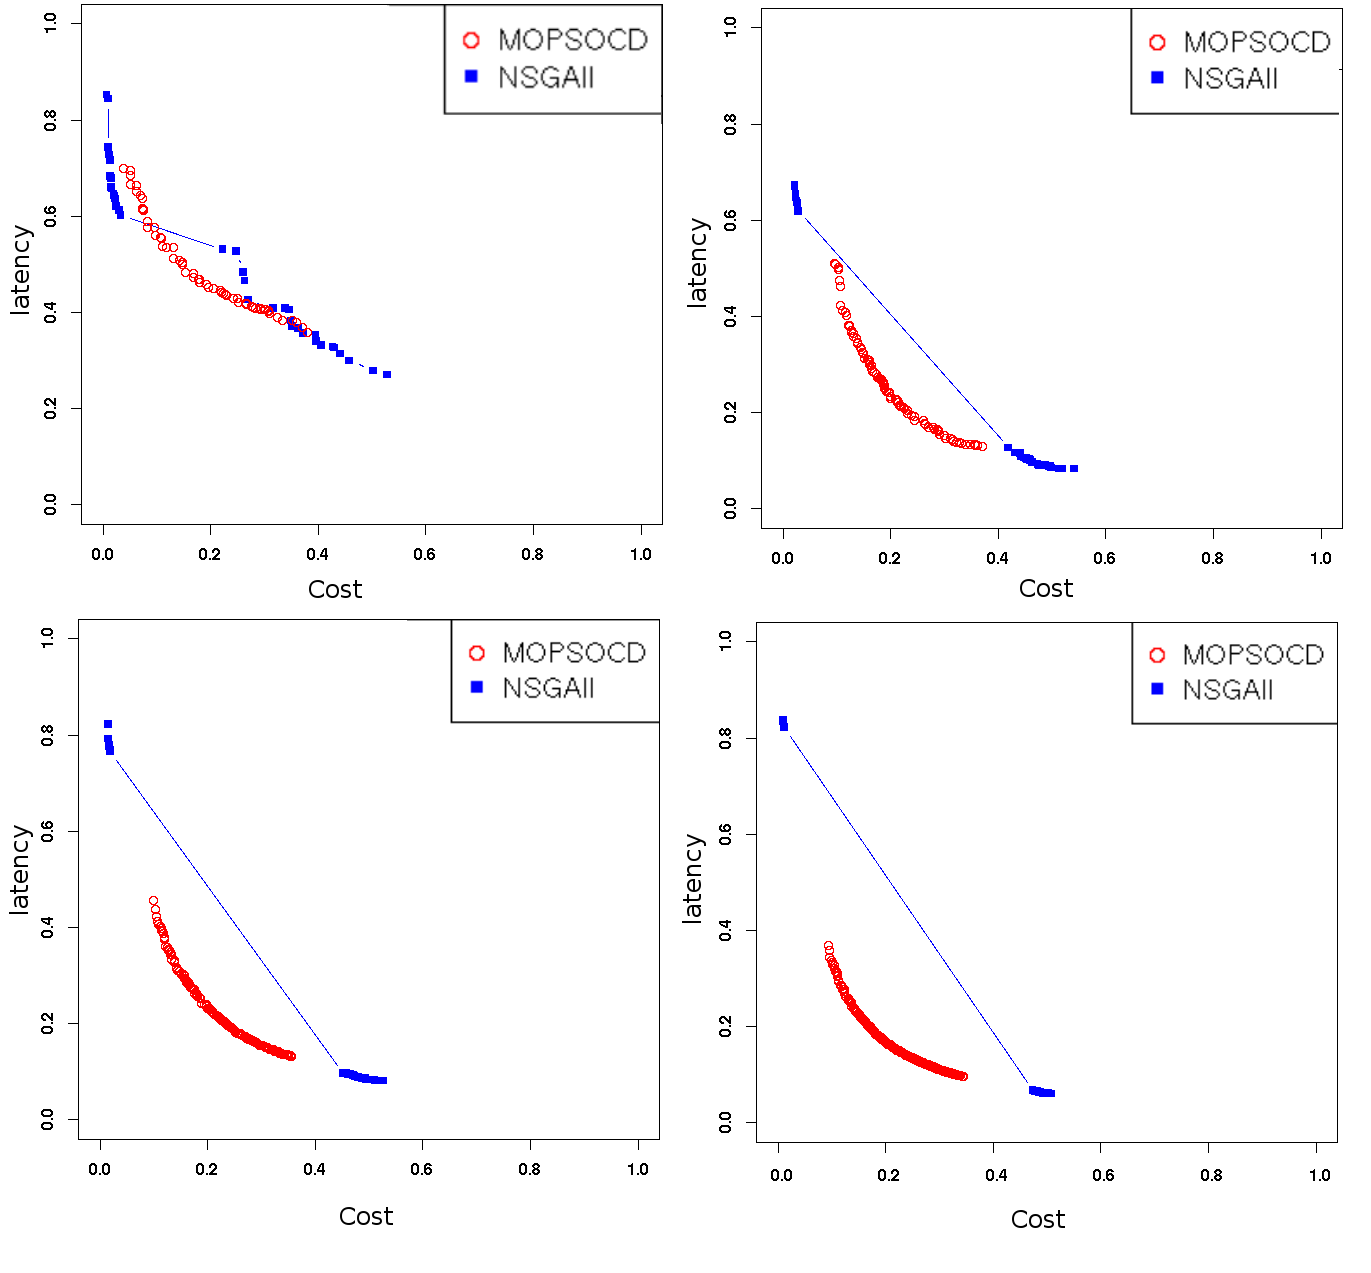
\includegraphics[width=\textwidth]{pics/1.png}
	   \caption{Problem 1}
   \end{subfigure}
   \begin{subfigure}{0.4\textwidth}
       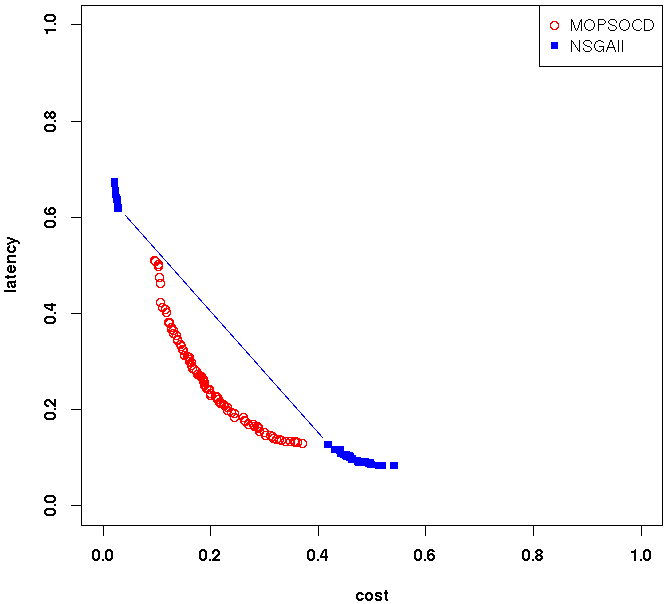
\includegraphics[width=\textwidth]{pics/2.png}
	   \caption{Problem 2}
   \end{subfigure}
   \begin{subfigure}{0.4\textwidth}
       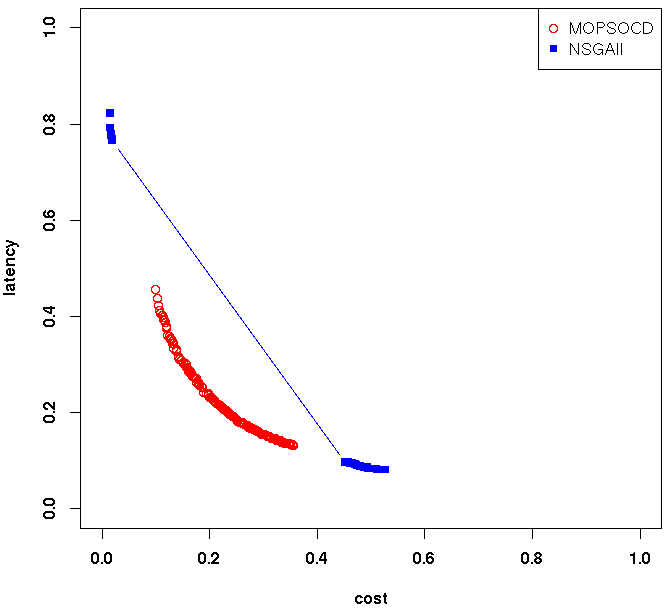
\includegraphics[width=\textwidth]{pics/3.png}
	   \caption{Problem 3}
   \end{subfigure}
   \begin{subfigure}{0.4\textwidth}
       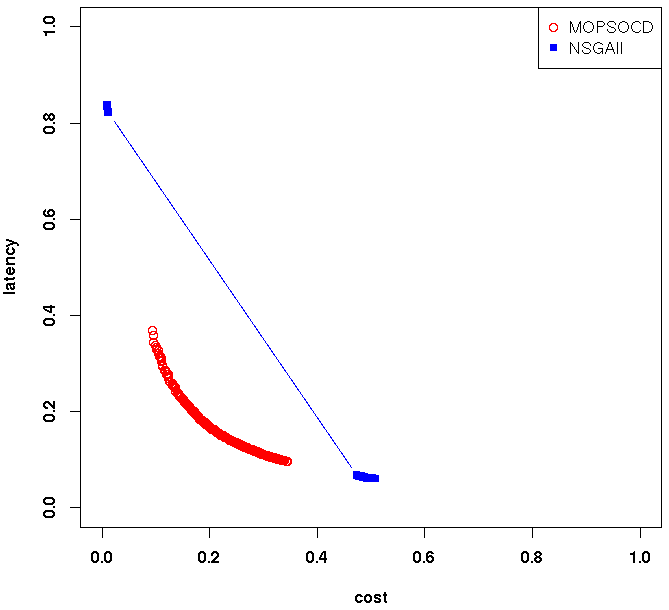
\includegraphics[width=\textwidth]{pics/4.png}
	   \caption{Problem 4}
   \end{subfigure}
   \caption{Experimental results}
   \label{fig:results}
\end{figure}


It is easy to notice that in the first two problems, the number of variable are relatively small. 
Both algorithms were able to handle the problem and generated a Pareto front. In both test cases,
MOPSOCD presents better results. In terms of quality, the Pareto front generated by MOPSOCD is clearly under the NSGA-II 
which means its closed to optimal solution. In terms of distribution, Pareto front of MOPSOCD is well-distributed along
with the true Pareto front. Although in some cases, it sacrificed quality (e.g., upper part of problem 1). On the other
hand, NSGA-II form a nonuniform Pareto front.

In the last two problems, the number of variable are huge. Both algorithms show 
limitations on such scale of variables. As the results show, NSGA-II try to keep diversity in the solution set. As 
a consequence, the solution set shows polarity among solutions. This is certainly an undesirable solution. In constrast,
the result from MOPSOCD shows relatively good coverage of optima Pareto front.
%In the last two experiments, the number of variable are huge, 4000 and 16,000 respectively. Both algorithms could not 
%handle well and provided poor results. As the figure illustrates, Pareto front of NSGA-II is completely separated, 
%MOPSOCD failed to form a scattered Pareto front, because of the huge search space, the continuous Pareto front 
%looks like concentrated on an area. In these cases, both algorithms stuck at local optima.

The efficiency of the two algorithms with the results shown in Table \ref{table:time}. 

\begin{table}[h]
		\caption{Execution Time (s)}
		\scalebox{0.65}{
		\begin{tabular}{|1|1|l|l|l|l|l|l|l|l|l|}
		\hline
	 \multicolumn{2}{|l|}{problem 1} & \multicolumn{2}{l|}{problem 2} & \multicolumn{2}{l|}{problem 3} & \multicolumn{2}{l|}{problem 4} \\ \hline
		 MOPSOCD(s)	&	NSGA-II(s)	& 	MOPSOCD(s)	& 	NSGA-II(s)	&  	MOPSOCD(s)	&  	NSGA-II(s)	& 	MOPSOCD(s)	&   NSGA-II(s)\\ \hline
	   20.6347 $\pm$ 0.27		$\uparrow$ & 32.79 $\pm$ 0.59  &110.26 $\pm$ 0.70 $\uparrow$  &323.49 $\pm$9.13      &533.72 $\pm$ 8.63    $\uparrow$      & 2064.127 $\pm$69.65          &3416.83 $\pm$ 244.03  $\uparrow$         &  18980.26$\pm$801.454         \\ \hline
\end{tabular}
}
\label{table:time}
\end{table}

As the result shows, MOPSOCD is clearly much efficient than NSGA-II in every test case. 
Specifically, NSGA-II roughly takes 4 times longer than MOPSOCD in problem 3 and problem 4. 


